\documentclass{article}
\usepackage[utf8]{inputenc}
\usepackage{graphicx}
\usepackage{subfigure}
\usepackage{float}
\usepackage[pdfborder={0 0 0}]{hyperref}
\usepackage{color}
\definecolor{darkblue}{rgb}{0,0,.5}
\hypersetup{pdftex=true, colorlinks=true, breaklinks=true, linkcolor=darkblue, menucolor=darkblue, pagecolor=darkblue, urlcolor=darkblue, filecolor=darkblue}
\begin{document}
%\definecolor{darkblue}{rgb}{0,0,.5}
%hypersetup{pdftex=true, colorlinks=true, breaklinks=true, linkcolor=darkblue, menucolor=darkblue, pagecolor=darkblue, urlcolor=darkblue}

\title{RAxML-Workbench Help}

\date{}
\maketitle
\tableofcontents

\section{Main Menu Bar}
	\subsubsection*{New Submission}Switch to the Submission-section to use RAxML or other tools provided.
    \subsubsection*{Open Job}Open an older RAxML Job directory (RAxML\_info file has to be present) and open it within the GUI for further analysis.
    \subsubsection*{Open file in Treeviewer}Display a treefile in \underline{PhyloXML} format in the Treeviewer.
    \subsubsection*{Preferences} 
   		 \underline{Enable Uclust:}
 		\begin{itemize}
 			\item[] Download RC Edgar's \textit{uclust}(usearch) from \href{www.drive5.com/usearch/}{www.drive5.com/usearch/}. Select the uclust executable binary with the given file browser. You can also specify the identity level for the clusters in the field "Cluster Identity". Save your changes with the "Save" Button. If your configuration was valid, then the "Cluster Reads" Option within the EPA-Submission forms should be enabled.
 		\end{itemize}
 		\textcolor{red}{Attention!} It might happen that programs change their input specifications with new versions. We try to keep track of this, but if you encounter problems feel free to contact us (Please send us also the version of the program you used).
\section{The Submission-section}
	\begin{figure}[htb]
		\centering
		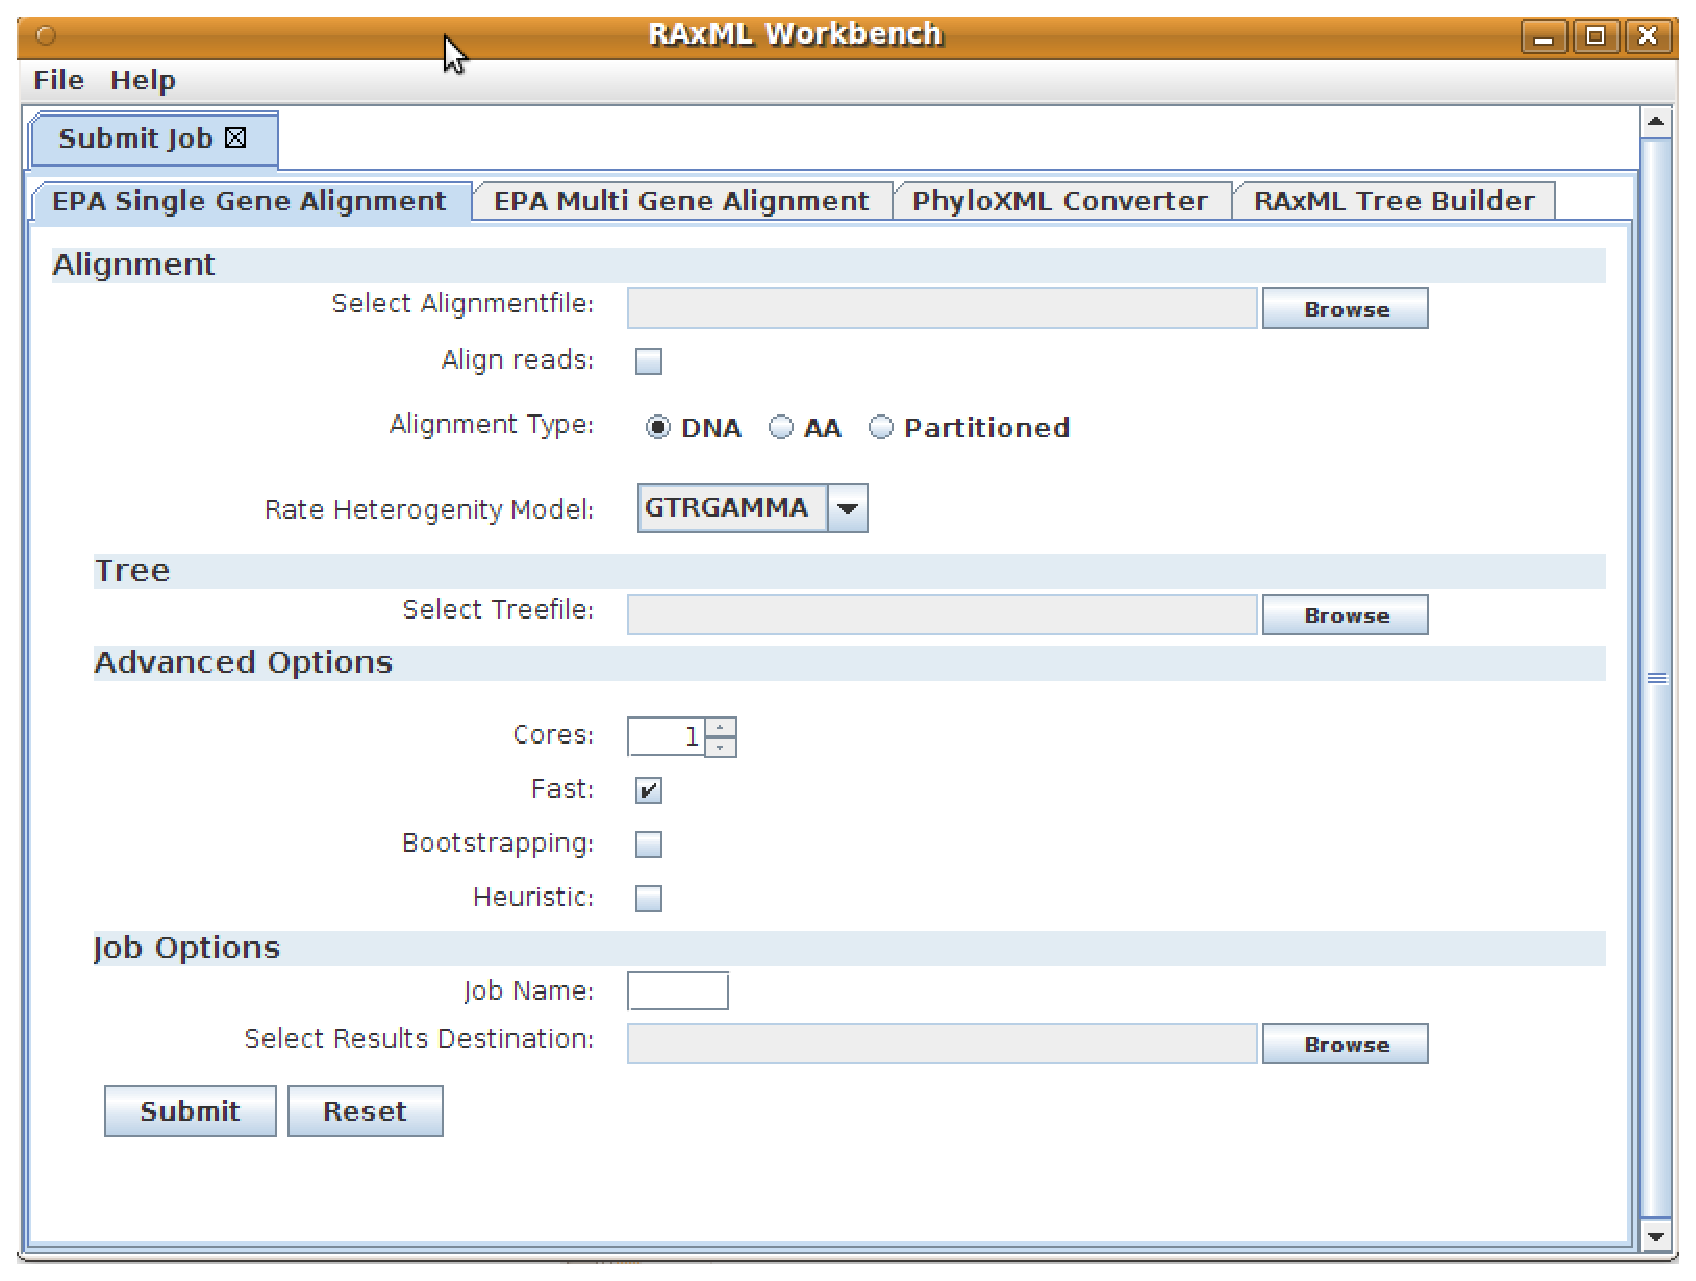
\includegraphics[scale=0.30]{./Submission}
		\caption{The Submission-section}
		\label{fig1}
	\end{figure}
	\noindent In this Section of the RAxML Workbench, you can run RAxML or other tools. 	
	\subsection{RAxML-EPA - Single Gene Alignment}
	The RAxML-EPA-Pipeline for Single Gene Alignment-files. The first 4 parameters must be entered to let the EPA run:
	\subsubsection*{Alignmentfile}
	Select a reference alignment with aligned query sequences in FASTA or PHYLIP format. If the query sequences are not aligned to the reference alignment, you can check the \textit{Upload unaligned reads} button below and select the query reads separately. The program will automatically rename taxa if they are not unique within the alignment due to PHYLIP format conversion tools that restrict taxa names to 10 characters only.
	\subsubsection*{Treefile}
	Select an unrooted, strictly bifurcating reference tree in Newick format that contains the reference sequences. The tree does not need to contain branch lengths because they will be automatically estimated by the RAxML EPA algorithm.
	\subsubsection*{Results Destination}
	Select the parent folder where the RAxML Workbench is going to save your results.
	\subsubsection*{Jobname}
	Enter the name of the folder where RAxML is going to save your results. \\\\
	There are more optional parameters available:
	\subsubsection*{Align Reads}
	Check this box if you want the program to automatically align your reads to the full-length reference sequence alignment using \textit{hmmalign}. In the case that you have a huge number of reads you may then also chose the option \textit{Cluster reads} (if enabled, see Preferences). The aligning is then only performed for consensus reads that are built using RC Edgar's \textit{uclust} program.   
	\subsubsection*{Cores}
	If you have more than one core available you can increment this number to perform the parallel version of RAxML on your local machine.
	\subsubsection*{Alignment Type}
	 Select the type of data in your alignment, this can be either DNA or Protein data or any combination of DNA, Protein, Secondary Structure, Multi-State, or Binary data partitions as specified by a standard RAxML partitioned model file (passed vie the -q option).
	 \subsubsection*{Bootstrapping}
	 Check this button if you want to infer query placement uncertainty values via standard phylogenetic Bootstrapping.
	 \subsubsection*{Heuristic}
	  Check this box if you want to use the fast placement heuristics (recommended for large datasets).
		
	\subsection{RAxML-EPA - Multi Gene Alignment}
		The RAxML-EPA-Pipeline for Multi Gene Alignment-files. The first 6 parameters must be entered to let the EPA run:
		\subsubsection*{Alignmentfile}	
			Select a reference alignment with aligned query sequences in FASTA or PHYLIP format. If the query sequences are not aligned to the reference alignment, you can check the \textit{Upload unaligned reads} button below and select the query reads separately. The program will automatically rename taxa if they are not unique within the alignment due to PHYLIP format conversion tools that restrict taxa names to 10 characters only.
		\subsubsection*{Treefile}
			Select an unrooted, strictly bifurcating reference tree in Newick format that contains the reference sequences. The tree does not need to contain branch lengths because they will be automatically estimated by the RAxML EPA algorithm.
		\subsubsection*{Multi Gene Partitionfile}
		Select a partitionfile that tells RAxML how the alignment is separated into the different genes. 
		\subsubsection*{Readsfile}	
		Select file containing the reads in FASTA format that have to be aligned. The program will assign the reads to the most fitting gene based on the Smith-Waterman algorithm. The reads are then aligned with \textit{hmmalign}. In the case that you have a huge number of reads you may then also chose the option \textit{Cluster reads} (if enabled, see Preferences). The aligning is then only performed for consensus reads that are built using RC Edgar's \textit{uclust} program.
		\subsubsection*{Results Destination}
			Select the parent folder where the RAxML Workbench is going to save your results.
		\subsubsection*{Jobname}
			Enter the name of the folder where RAxML is going to save your results. \\\\
	There are more optional parameters available:
		\subsubsection*{Cores}
			If you have more than one core available you can increment this number to perform the parallel version of RAxML on your local machine.
	 	\subsubsection*{Bootstrapping}
	 		Check this button if you want to infer query placement uncertainty values via standard phylogenetic Bootstrapping.
	 	\subsubsection*{Heuristic}
	  		Check this box if you want to use the fast placement heuristics (recommended for large datasets).	
		
	\subsection{Generate PhyloXML files}
		This tool can generate PhyloXML formated files from your (older) RAxML results, that can be displayed in the treeviewer. The program needs three input parameters to run.
		\subsubsection*{RAxML Classificationweights}
			Select a RAxML\_classificationLikelihoodWeights.-File, a RAxML\_classification.-File in case you performed RAxML with bootstrapping or another file that has also 4 columns where the first column is the sequence-name, the second the branch-name, the third the likelihood weight and the fourth the sum of the likelihood weights listed above from the same sequence.
		\subsubsection*{Reference Tree}
			Select the unrooted, strictly bifurcating reference tree in Newick format on which the RAxML-EPA algorithm performed the placements listed in the corresponding classificationfile selected above.
		\subsubsection*{Destination path}
		Simply specify where the resulting PhyloXML file should be saved.
		
	\subsection{RAxML Tree Builder}
		RAxML (Randomized Axelerated Maximum Likelihood) is a program for sequential and parallel Maximum Likelihood based inference of large phylogenetic trees. The first 3 parameters must be entered to let RAxML run:
		\subsubsection*{Alignmentfile}
			Select a reference alignment with aligned query sequences in FASTA or PHYLIP format. If the query sequences are not aligned to the reference alignment, you can check the \textit{Upload unaligned reads} button below and select the query reads separately. The program will automatically rename taxa if they are not unique within the alignment due to PHYLIP format conversion tools that restrict taxa names to 10 characters only.
		\subsubsection*{Results Destination}
			Select the parent folder where the RAxML Workbench is going to save your results.
		\subsubsection*{Jobname}
			Enter the name of the folder where RAxML is going to save your results. \\\\
			There are more optional parameters available:
		\subsubsection*{Cores}
			If you have more than one core available you can increment this number to perform the parallel version of RAxML on your local machine.
		\subsubsection*{Parsimony Random Seed}
			Specify a random number seed for the parsimony inference.
		\subsubsection*{Alignment Type}
	 		Select the type of data in your alignment, this can be either DNA or Protein data or any combination of DNA, Protein, Secondary Structure, Multi-State, or Binary data partitions as specified by a standard RAxML partitioned model file (passed vie the -q option).
	 	\subsubsection*{Bootstrapping}
			 Check this button if you want RAxML to perform a bootstrap analysis.
\section{The Results-section}
\begin{figure}[htb]
		\centering
		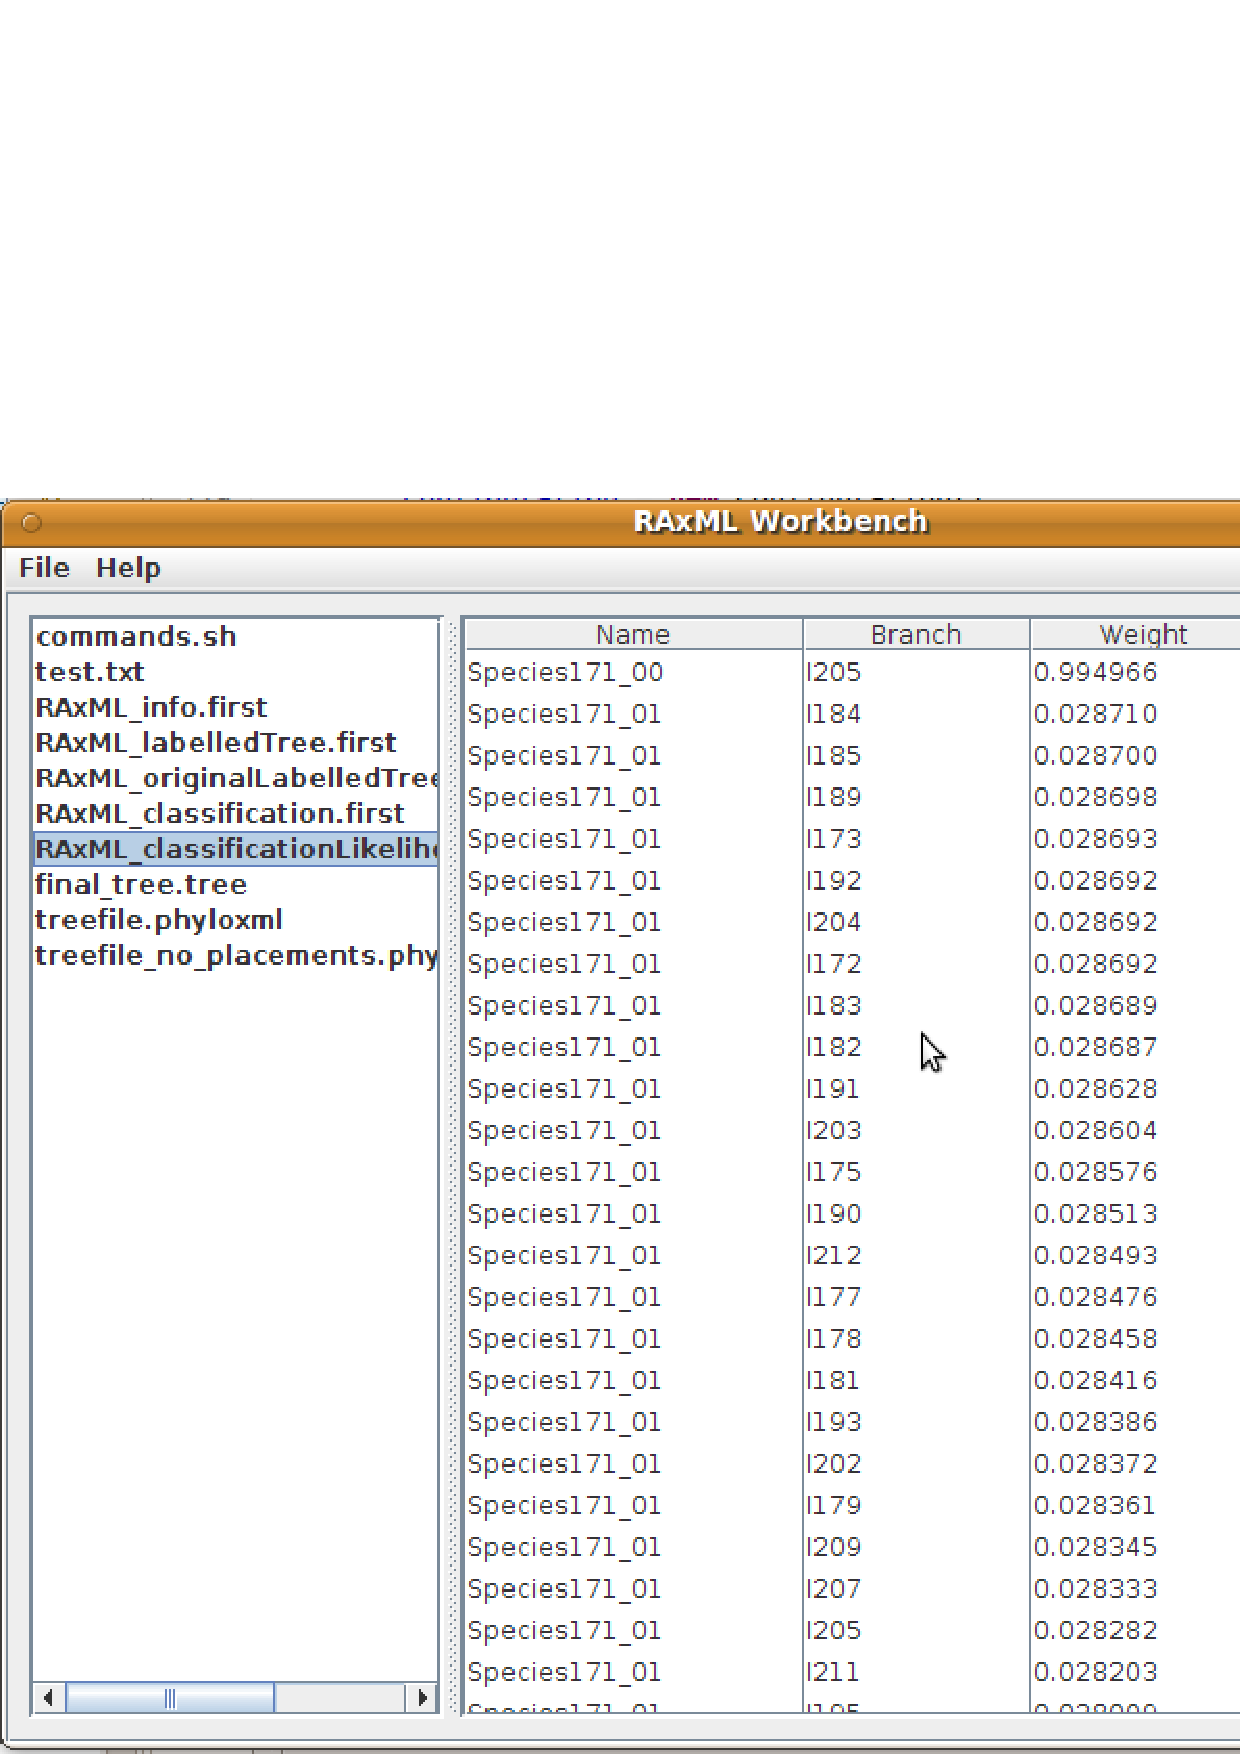
\includegraphics[scale=0.30]{./Results}
		\caption{The Results-section}
		\label{fig2}
	\end{figure}
		\noindent On the left-hand side, all available files within the selected RAxML job-folder are displayed. The content of the files is shown in the right panel when clicking on it. Classificationfiles are displayed as tables and PhyloXML formated files are directly displayed in the treeviewer. Every other file is displayed as plain text.
	
\section{The Treeviewer}
	\begin{figure}[htb]
		\centering
		\includegraphics[scale=0.3]{./overview_treeviewer}
		\caption{The Archaeopteryx Treeviewer}
		\label{fig3}
		\end{figure}
    \noindent We provide a brief overview of some relevant Archaeopteryx Treeviewer features below.
	For a more detailed description, please refer to the Archaeopteryx project web-site http://www.phylosoft.org/archaeopteryx\\
    \underline{Attention!} The features listed below are not part of the original Archaeopteryx treeviewer and were added subsequently:
    \begin{itemize}
        \item Colorize Branches with different scorings
        \item Mouse rollover histograms
        \item Branchdata pop-ups
        \item Branch labels
        \item Node width
     \end{itemize}
      If you have questions, proposals or other concerns regarding these points, feel free to contact us. 
    	
   
        \subsection{Left Checkboxes(1)}
        \subsubsection*{Phylogram} The  branch lengths of the tree correspond to the branch length given within the tree.
        \subsubsection*{Dyna Hide} Dynamically hide labels if not enough space is available.
        \subsubsection*{Rollover} Activates the mouse over function for the tree. 
        \subsubsection*{Colorize Branches} Assign colors to branches based on diversity measures. The coloring represents the mean value of the confidences off all placements on that branch. The confidences correspond to the diversity scorings selected beneath.
        \begin{itemize}
       		\item \textit{QSBI:} - A prototype diversity measure that scores for every branch, if the placements distribution in the left and right subtree of a query sequence is better than expected. The mean of all query sequences is taken as score. Green means that the placement distributions in the left and right subtree is significantly different from what has been expected.
        	\item \textit{EDPL:} - Measures the spreading of the query sequence within the tree. A brighter green means a very high mean confidence on that branch. A bright red means the opposite. The slider allows a manual adjustment of the cutoff.
        \end{itemize}
        All measurements can be combined. 
        \subsubsection*{Use Branch-Width} Display the fraction of reads that have been placed into a branch by means of a relative branch width.
        \subsubsection*{Use Node-Width} Display the fraction of reads that have been placed in the underlying subtree by means of a relative node width.
        \subsubsection*{Leaf Names} Display the taxa names on the leaves of the tree.
        \subsubsection*{Branch Names} Display the branch labels.
 	 \subsection{Tree-manipulation(2)}
        In the drop down menu below "Click on Node to:" you can switch between actions that are performed when you click on a node or a branch in the visualized tree respectively.
          \begin{itemize}
              \item Display Node Data
              \item Collapse/Uncollapse
              \item Root/Reroot (only on branches)
              \item Sub/Super Tree
              \item Swap Descendants
              \item Colorize subtree
              \item Delete Subtree/Node
           \end{itemize}
       \subsection{Top main panel}
          \subsubsection*{Type:}
          Select your preferred tree layout between the following:
          \begin{itemize}
              \item Rectangular
              \item Euro Type
              \item Rounded
              \item Triangular
              \item Unrooted
          \end{itemize}   
          \subsubsection*{View as Text:}
          View the represented tree in different file formats like e.g. phyloXML
       
       \subsection{The interactive tree visualization}
          \subsubsection*{Branch placement histogram(3)}
          A mouse roll over on a branch that has placements on it displays a histogram of RAxML weights. These weights represent either likelihood weights or bootstrap supports.  
          \subsubsection*{Branch Data View(4)}
          By left clicking on a branch, a pop up window is displayed showing a more detailed view of the placements present on the corresponding branch. In the bottom part of the window, a table with the read names, the EDPL scores and the RAxML weights (likelihood or bootstrap support) are displayed. \\
\end{document}